\documentclass{article}

\usepackage{nips_2018}

\usepackage[T1]{fontenc}    % use 8-bit T1 fonts

% Useful packages
\usepackage{amsmath, amssymb, amsfonts, bm}
\usepackage{amsthm}
\usepackage{booktabs}       % professional-quality tables
\usepackage{mathtools}
\usepackage{nicefrac}       % compact symbols for 1/2, etc.
\usepackage[usenames, dvipsnames]{color}
\usepackage{multirow}
\usepackage{hyperref}

\usepackage{floatrow}
\floatsetup[table]{capposition=top}

\usepackage{wrapfig}
\usepackage{multicol}

% For gap between cmidrules.
\usepackage{array}
\newcolumntype{C}{@{\extracolsep{0.1cm}}c@{\extracolsep{0pt}}}%

\setlength{\columnsep}{1cm}
\setlength{\columnseprule}{0.5pt}
\def\columnseprulecolor{\color{Plum}}

% Simple macros.
\def\sec#1{Sec.~\ref{#1}}
\def\Sec#1{Sec.~\ref{#1}}
\def\fig#1{Fig.~\ref{#1}}
\def\Fig#1{Fig.~\ref{#1}}
\def\tableref#1{Table~\ref{#1}}

\newcommand{\tk}[1]{\textcolor{red}{TK: #1}}
\newcommand{\tkf}[1]{\footnote{\tk{#1}}}
\newcommand{\ao}[1]{\textcolor{green}{AO: #1}}
\newcommand{\tsj}[1]{\textcolor{magenta}{TSJ: #1}}
\newcommand{\vm}[1]{\textcolor{blue}{Vincent M: #1}}
\newcommand{\vmf}[1]{\footnote{\vm{#1}}}


\newcommand{\cw}{\mathbf{cw}}
\newcommand{\cc}{\mathbf{c}}
\newcommand{\kb}{\mathbf{k}}
\newcommand{\mem}{\mathbf{m}}
\newcommand{\rr}{\mathbf{r}}

\title{On transfer learning using a MAC model variant: supplementary material}

% The \author macro works with any number of authors. There are two
% commands used to separate the names and addresses of multiple
% authors: \And and \AND.
%
% Using \And between authors leaves it to LaTeX to determine where to
% break the lines. Using \AND forces a line break at that point. So,
% if LaTeX puts 3 of 4 authors names on the first line, and the last
% on the second line, try using \AND instead of \And before the third
% author name.

\author{
	\textbf{\null\hfill Vincent Marois \hfill T.S. Jayram \hfill Vincent Albouy  \hfill\null}\\
	\textbf{\null\hfill Tomasz Kornuta \hfill Younes Bouhadjar \hfill Ahmet S. Ozcan \hfill\null}\\
	IBM Research AI, Almaden Research Center, San Jose, USA\\
	\texttt{\{vmarois,jayram,tkornut,byounes,asozcan\}@us.ibm.com}\\
	\texttt{\{vincent.albouy\}@ibm.com}\\
}

\begin{document}
% \nipsfinalcopy is no longer used

\maketitle

% Little cheating to make our names fit:]
\vskip -0.5cm
\begin{abstract}
We introduce a variant of the MAC model (Hudson and Manning, CVPR 2018) with a simplified set of equations that achieves comparable accuracy, while training faster. We evaluate both models on CLEVR and CoGenT, and show that, transfer learning with fine-tuning results in a 15 point increase in accuracy, matching the state of the art. Finally, in contrast, we demonstrate that improper fine-tuning can actually reduce a model's accuracy as well.
\end{abstract}
\section{Introduction}
Reasoning over visual inputs is a fundamental characteristic of human intelligence.
Reproducing this ability with artificial agents is a challenge that requires learning relations and compositionality (Hu et al. 2017; Johnson et al. 2017b).

The Visual Question Answering (VQA) task has been tailored to benchmark those reasoning performances. It is a complex semantic task requiring both natural language processing and visual recognition. It also puts to the test the effective use of the short term memory.

The recent CLEVR dataset (Johnson et al., 2017a) proposes a challenging multimodal task that requires to answer compositional questions about an image. The dataset is designed with the explicit goal of enabling detailed analysis of visual reasoning.
Solving this problem involves a broad array of skills such as counting, comparison and understanding transitive reasoning.
It also requires perceptual abilities such as recognizing objects, attributes, and spatial relations as well as leveraging commonsense world knowledge (Hudson et al. 2018).
CLEVR is a generated synthetic dataset that allows to introduce variations on a subset of data to test a particular ability such as generalization or transfer learning.

To solve this type of reasoning task, many deep learning approaches have been explored although they often struggle to perform well on tasks with a structured and compositional nature (Garnelo et al., 2016; Lake et al., 2017). 
More recent approaches adopt modular structures, resembling the trees of programming languages, that compose neural modules from a fixed predefined collection (Andreas et al., 2016a; Johnson et al., 2017b, Mascharka et al., 2018). However, they rely on externally provided structured representations and functional programs, parsers or expert demonstration, and sometimes require reinforcement learning training schemes (Hudson et al. 2018). 
These models’ structure is inherently rigid and the use of a range of specialized modules weaken their robustness and generalization capacities.

Recent work on CLEVR from Hudson et al. 2018;  has introduced  MAC ( Memory, Attention, and Composition). The MAC model has been deliberately designed to decompose the problem into a sequence of attention-based reasoning operations. Its ability to arbitrarily draw a complex reasoning graph while still featuring end-to-end differentiability made its sucess.
MAC doesn’t use specific modules that would make it specifically tailored for the CLEVR dataset. The three general units working in tandem to perform a reasoning step make the robustness of the model.

MAC achieves state-of-the-art accuracy on CLEVR and also on the most difficult CLEVR Humans dataset, were questions are written by humans. 
Although the performance of MAC has been proven, It appears difficult to understand what concepts the model is learning. 
Does the model really learn relations between objects? 
How does the model represent those relations and reasoning steps? 
The interpretability of the MAC model seems yet to be fully defined.
Is the model representing notions and concepts like objects attributes?

In this work, we first question the complexity of the MAC model and explore simplification possibilities. We propose a new set of equations that aims to simplify the model and improve training performance. 
We also put to proof the MAC model on the CLEVR CoGenT dataset. The CoGenT dataset has been designed to highlight transfer learning abilities and give a better sense of interpretability. By mixing attributes over two sub-datasets, the CLEVR CoGenT task allow us to see what relations and concepts the model has really learned. We show how MAC performs on CLEVR CoGenT and compare it to state-of-the-art models and propose a study about the model failures. This work points out some of the MAC model weaknesses, in particular its failure to differentiate concepts of colors and shape. We finally discuss some improvement possibilities.

\section{Description of MAC model}


A MAC network is an end-to-end differentiable architecture primed to perform an explicit multi-step reasoning process, by stringing together p recurrent MAC cells, each responsible for performing one reasoning step. Given a knowledge base K (for VQA, an image) and a task description q (for VQA, a question), the model infers a decomposition into a series of p reasoning operations that interact with the knowledge base, iteratively aggregating and manipulating information to perform the task at hand. It consists of three components: (1) an input unit, (2) the core recurrent network, composed out of p MAC cells, and (3) an output unit, all described below.

\begin{figure}[htbp]
	\centering
	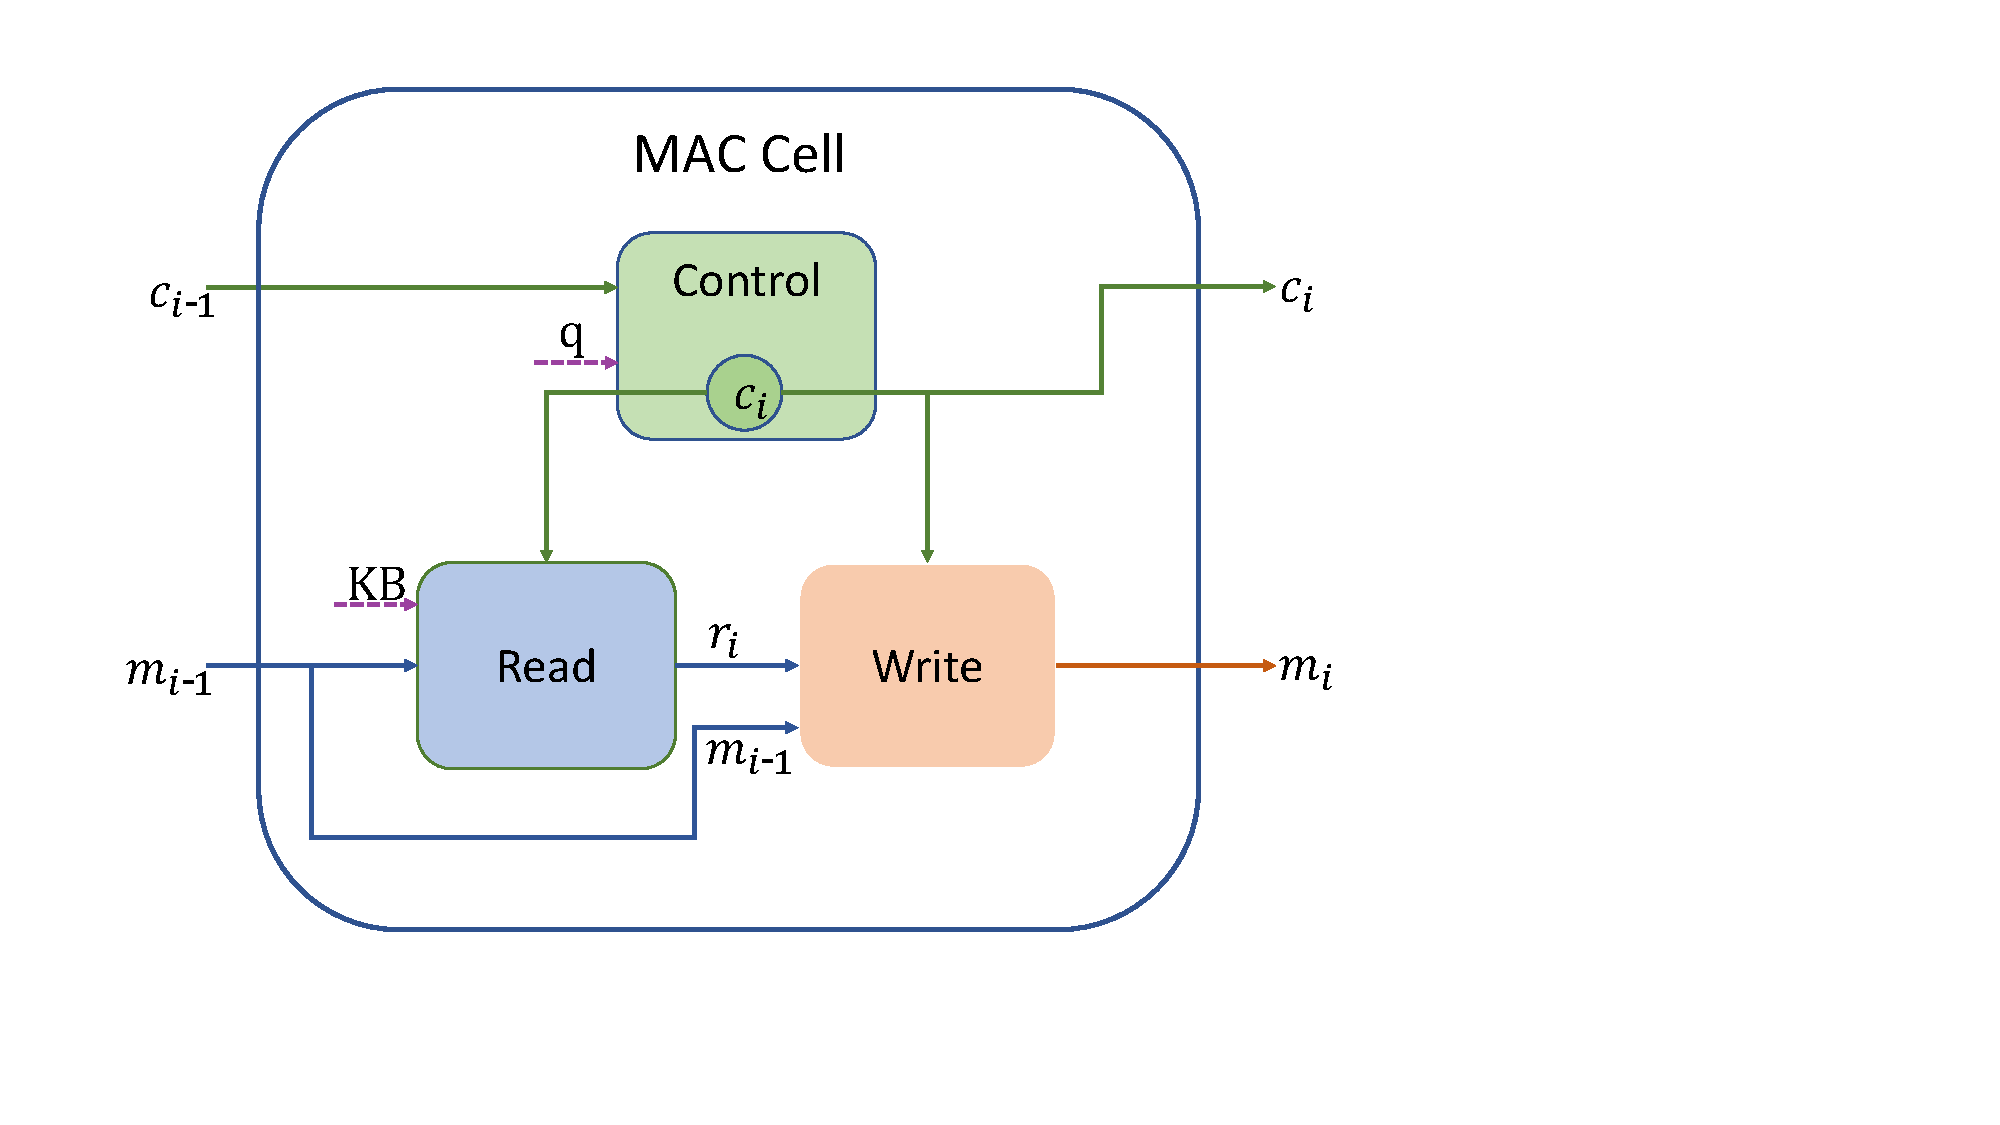
\includegraphics[width=0.7\textwidth]{img/mac_cell.pdf}
	\caption{The Mac Cell. The MAC recurrent cell consists of a control unit, read unit, and write unit, that operate over dual control and memory hidden states. The control unit successively attends to different parts of the task description (question), updating the control state to represent at each timestep the reasoning operation the cell intends to perform. The read unit extracts information out of a knowledge base (here, image), guided by the control state. The write unit integrates the retrieved information into the memory state, yielding the new intermediate result that follows from applying the current reasoning operation.}
	\label{fig:core_concepts}
\end{figure}


\subsection{Simplified MAC network}
Our proposed modification to the MAC network is based on two heuristic
simplifications of the equations governing a MAC cell. 
First, we observed that when looking at the equations of different units
together as a whole, we notice that there are several affine transformations
that are applied in sequence (with no activation in-between).
Therefore they can actually be combined to form a single affine transformation.
The second observation uses the following heuristic argument:
suppose there is a single affine transformation which preserves the number
of dimensions. Then one can assume that the transformation is invertible
so as to avoid a loss in the information. Applying this principle to 
equations in the read and write unit results in eliminating an affine
operation of the knowledge base in the recurrent network. Instead we compute
this operation on the knowledge base right after we apply the 2 
trainable CNN layers (i.e. prior to the reasoning steps). This results
in a significant savings in training time, as our experiments demonstrate
below, without incurring too much drop in accuracy.

In the description below, the original MAC cell equations are shown on the \emph{left}
while our simplified equations are shown (in color) on the {\color{Plum} \emph{right}}.
(The equation numbering is the same as in~\cite{hudson2018compositional}.)

\noindent\textit{Notation:} The index/position $i$ below denotes the reasoning step. 
Unless mentioned otherwise, the weights/biases are invariant w.r.t $i$, 
i.e., shared across all the reasoning steps. 

\noindent\textbf{Control unit:} 
For both models, in the control unit, the question $q$ is first transformed in each step of 
%the reasoning using a \emph{position-aware}~\cite{hudson2018compositional} 
linear layer: $q_i = U_i^{[d \times 2d]} q + b_i^{[d]}$.

\begin{multicols}{2}
	\noindent
	\begin{align*}
	&cq_i = W_{cq}^{[d \times 2d]} [c_{i-1}, q_i] + b_{cq}^{[d]}  \tag{c1} \\
	&ca_{is} = W_{ca}^{[1 \times d]} (cq_i \odot \cw_s) + b_{ca}^{[1]}
	\tag{c2.1}\\
	&cv_{is} = \textrm{softmax}(ca_{is}) \tag{c2.2}\\
	&\cc_i = \sum_s cv_{is} \, \cw_s  \tag{c2.3}
	\end{align*}
	\columnbreak
	{\color{Plum}
	\begin{align*}
	&cq_i = W_{cq}^{[d \times d]} c_{i-1} + q_i  \tag{c1} \\
	&ca_{is} = W_{ca}^{[1 \times d]} (cq_i \odot \cw_s)  \tag{c2.1}\\
	&cv_{is} = \textrm{softmax}(ca_{is}) \tag{c2.2}\\
	&\cc_i = \sum_s cv_{is} \, \cw_s  \tag{c2.3}
    \end{align*}}
\end{multicols}

\noindent\textbf{Read and write units:}
For both models below, $\kb_{hw}$ denotes the 
\emph{knowledge base}~\cite{hudson2018compositional}
consisting of 3D tensors with dimension $H \times W \times d$ for each image
in the data set. The difference in computing $\kb_{hw}$ is that the simplified MAC uses
an additional linear layer on top of the 2 CNN layers present in the original MAC network.
This circumvents the need for performing additional linear transformations on the 
knowledge base, as is done by the original MAC network in \emph{each} reasoning step.

\begin{multicols}{2}
	\noindent
	\begin{align*}
	&I_{ihw} = (W_{m}^{[d \times d]} \mem_{i-1} + b_{m}^{[d]}) \\
	           & \qquad \quad \odot (W_{k}^{[d \times d]} \kb_{hw} + b_{k}^{[d]}) \tag{r1} \\
	&I'_{ihw} =  W_{I'}^{[d \times 2d]} [I_{ihw},\kb_{hw}]  + b_{I'}^{[d]}  \tag{r2} \\
	&ra_{ihw} = W_{ra}^{[1 \times d]} (\cc_i \odot I'_{ihw}) + b_{ra}^{[1]} \tag{r3.1}\\
	&rv_{ihw} = \textrm{softmax}(ra_{ihw}) \tag{r3.2}\\
	&\rr_i = \sum_s rv_{ihw} \, \kb_{hw}  \tag{r3.3}\\
	&\mem_i = W_{rm}^{[d \times d]} [\rr_i, \mem_{i-1}]  + b_{rm}^{[d]} \tag{w1}	
	\end{align*}
	\columnbreak
	{\color{Plum}
	\begin{align*}
	&I_{ihw} = \mem_{i-1} \odot \kb_{hw} \tag{r1} \\ \\
	&I'_{ihw} = W_{I'}^{[d \times d]} I_{ihw} + b_{I'}^{[d]} + \kb_{hw} \tag{r2} \\
	&ra_{ihw} = W_{ra}^{[1 \times d]} (\cc_i \odot I'_{ihw})  \tag{r3.1}\\
	&rv_{ihw} = \textrm{softmax}(ra_{ihw}) \tag{r3.2}\\
	&\rr_i = \sum_s rv_{ihw} \, \kb_{hw}  \tag{r3.3}\\
	&\mem_i = W_{rm}^{[d \times d]} \rr_i + b_{rm}^{[d]} \tag{w1}
	\end{align*}}
\end{multicols}


\section{Experiments}

We evaluated SAMNet on the COG dataset~\cite{yang2018dataset}.
Our experiments were designed to study SAMNet's performance as well as its generalization abilities in different settings.
For this purpose, we used two different variants of the COG dataset: an easy one (Canonical) and a Hard version to explore a wide range of difficulties.
The main differences are the number of frames in the input sequence (4 vs. 8) and the maximum number of distractors (i.e., objects not relevant for the answer) per frame (1 vs. 10).
%More details on the dataset, its variants and tasks can be found in the Appendix.


%
%We compare our model to the original COG model  ~\cite{yang2018dataset} using their implementation (https://github.com/google/cog) and scores given by the authors. We also use the exact same training parameters detailed in the original paper.
%
%On the other side we trained SAMNet using IBM's Mi-Prometheus~\cite{kornuta2018accelerating}, a framework for research based on Pytorch. We trained all our models using NVIDIA’s GeForce GTX TITAN X GPUs. We trained  SAMNet using 8 reasoning steps SAMCells and a hidden state size of 128. The external memory has 128-bit slots. We trained our model until convergence but we also have set a training time limit of 80 hours.


\begin{figure}[htbp]
	\centering
  \begin{subfigure}{\textwidth}
    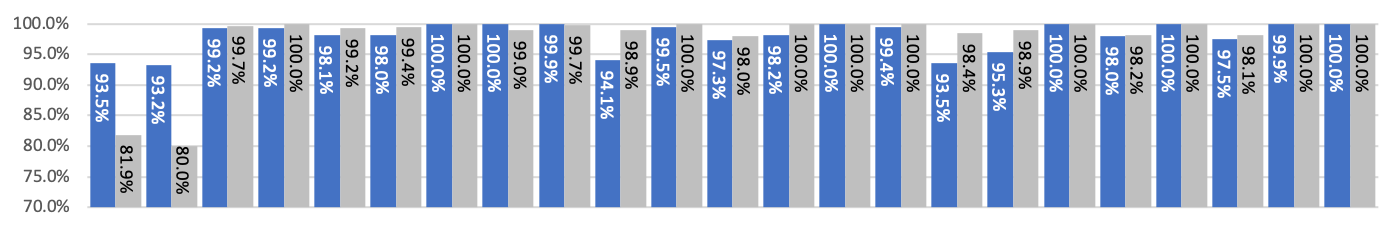
\includegraphics[width=0.92\textwidth]{../results/samnet_cog_orig_canonical_no_labels.png}
  \end{subfigure}%
  \newline
  \begin{subfigure}{\textwidth}
	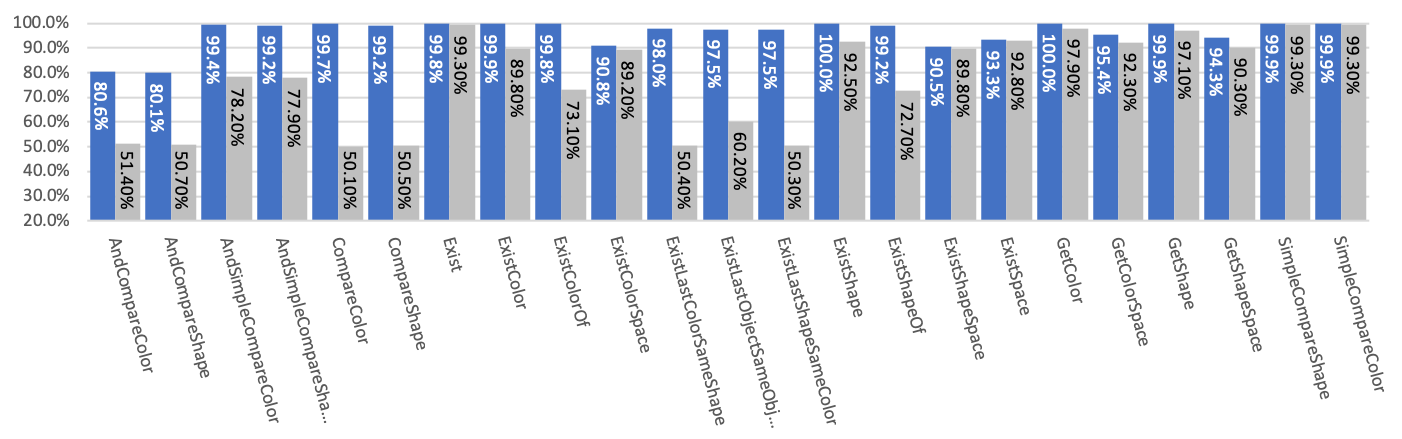
\includegraphics[width=0.93\textwidth]{../results/samnet_cog_orig_hard.png}
  \end{subfigure}%
\caption{Comparison of test set accuracies of SAMNet (blue) with original results achieved by the COG model (gray) on Canonical (top) and Hard (bottom) variants of the COG dataset.}
\label{fig:samnet_cog_detailed}
\end{figure}

\begin{figure}
	\centering
	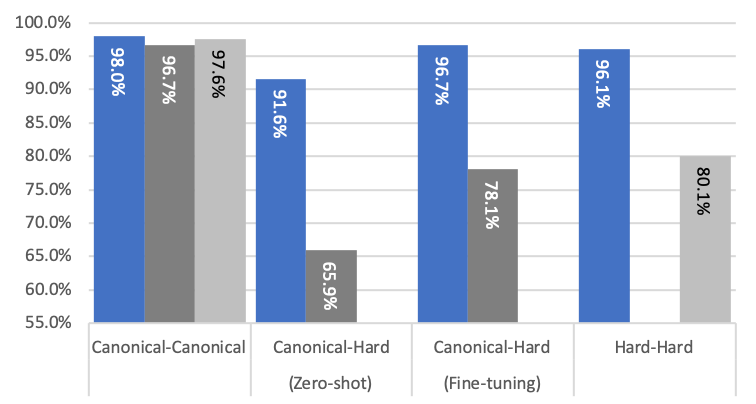
\includegraphics[width=0.75\textwidth]{../results/samnet_cog_overall_transfer.png}
	\caption{Total accuracies of SAMNet (blue) and COG models (light/dark gray) when testing generalization from Canonical to Hard variants of the dataset.}
	\label{fig:samnet_cog_overall_transfer}
\end{figure}

We have implemented and trained our SAMNet model using MI-Prometheus~\cite{kornuta2018accelerating}, a framework based on Pytorch~\cite{paszke2017automatic}. 
In our experiments, we have focused on 22 classification tasks and compared our results with the baseline model, as presented in \cref{fig:samnet_cog_detailed}.
For the Canonical variant (top row), we have achieved similar accuracies for the majority of tasks (with the total average accuracy of 98.0\% in comparison of 97.6\% achieved by the COG model), with significant improvements (around 13 points) for \textit{AndCompare} tasks.
As those tasks focus on compositional questions referring to two objects, we hypothesize that our model achieved better accuracy due to the ability to selectively pick and store the relevant objects from the past frames in the memory.
Despite there being some tasks in which our model reached slightly lower accuracies,
% (between 0.2 and 1.8 points)
when comparing performances on the Hard variant, it improves upon the  COG baseline on all tasks, with improvements varying from 0.5 to more than 30 points.

The goal of the next set of experiments was to test the generalization ability concerning the sequence length and number of distractors.
For that purpose, we have compared the accuracies of both models when trained on the Canonical variant and tested on Hard (\cref{fig:samnet_cog_overall_transfer}).
As the original paper does not include such experiments, we have performed them on our own.  The light gray color indicates the original results, whereas dark gray indicates the accuracies of COG models that we have trained (fine-tuning/testing) using the original code provided by the authors.
For sanity check, in the first column, we report both the best-achieved score and the score reported in the paper when training and testing on Canonical variant, without any fine-tuning.
In a pure \textit{transfer learning} setup (second column), our model shows enormous generalization ability, reaching 91.6\% accuracy on the test set.
We have also tested both models in a setup where the model trained on a Canonical variant underwent additional fine-tuning (for a single epoch) on the Hard variant (third column).
In this case, the SAMNet model also reached much better performance, and, interestingly, achieved better scores from the model trained and tested exclusively on the Hard variant.
In summary, the results clearly indicate that the mechanisms introduced in SAMNet  enable it to learn to operate independently of the total number of frames or number of distractions, and allow it to generalize to longer videos and more complex scenes. One other strength of SAMNet is its interpretability. Observing attention maps (see supplementary material) shows that SAMNet can effectively perform multi-step reasoning over questions and frames as intended. It also accurately classifies temporal contexts as designed. However we notice that the model can sometime discover alternative strategies that were not in the intended design but the answers are still correct. 

%we used the canonical (easy) and hard settings that alter the number of distractors and sequence length.  Since there was no baseline for these tests (train on canonical, test on hard), we ran our own experiments using the COG model provided by the authors.  SAMNet achieves the highest overall scores for all categories of experiments (\cref{fig:samnet_cog_overall_transfer}), especially for the tests run on the hard dataset.  Among the 22 classification tasks, we highlighted the two most difficult tasks that affect the overall score. 
%We argue that the generalization capability of SAMNet is mainly due to the dynamic frame-by-frame processing of the input sequence. 
%The mechanisms introduced in SAMCell learn to operate independently of the total number of frames and allow to generalize to longer video lengths.
%As shown in \cref{fig:samnet_cog_overall_transfer}, when trained on the easy dataset, SAMNet still performs 91.6\% when tested on the hard dataset, whereas COG drops from 97.6\% to 65.9\%   The visualization of the trained SAMNet model (see Appendix) indicates that the model learns the concept of time, helping it to control the flow of information from visual input to the memory.  Therefore, the memory is updated efficiently instead of storing all information across all frames.






\section{Conclusion}


%\appendix

\section{Description of datasets}

Most of the VQA datasets have strong biases. This allow models to learn strategies without reasoning about the visual input~\cite{Santoro2017ASN}.
The CLEVR dataset~\cite{johnson2017clevr} was developed to address those issues and come back to the core challenge of visual QA which is testing reasoning abilities.
CLEVR contains images of 3D-rendered objects; each image comes with a number of highly compositional questions that fall into different categories.
Those categories fall into 5 classes of tasks: Exist, Count, Compare Integer, Query Attribute and Compare Attribute. 
The CLEVR dataset consists of:
\begin{itemize}
\item 	A training set of 70k images and 700k questions,
\item	A validation set of 15k images and 150k questions,
\item	A test  set of 15k images and 150k questions about objects,
\item	Answers, scene graphs and functional programs for all train and val images and questions.
\end{itemize}
Each object present in the scene, aside of position, is characterized by a set of four attributes:
\begin{itemize}
\item 2 sizes: large, small,
\item 3 shapes: square, cylinder, sphere,
\item 2 material types: rubber, metal,
\item 8 color types: gray, blue, brown, yellow, red, green, purple, cyan,
\end{itemize}
resulting in 96 unique combinations.

Along with CLEVR, the authors~\cite{johnson2017clevr} introduced  CLEVR-CoGenT (Compositional Generalization Test, CoGenT in short), with a goal of evaluating how well the models can generalize, learn relations and compositional concepts.
This dataset is generated in the same way as CLEVR with two additional conditions.
As shown in \tableref{tab:cogent_conditions}, in Condition A all cubes are gray, blue, brown, or yellow, whereas all cylinders are red, green, purple, or cyan; in Condition B cubes and cylinders swap color palettes.
For both conditions spheres can be any colors.


The CoGenT dataset contains:
\begin{itemize}
\item	Training set of 70,000 images and 699,960 questions in Condition A,
\item	Validation set of 15,000 images and 149,991 questions in Condition A,
\item	Test set of 15,000 images and 149,980 questions in Condition A (without answers),
\item	Validation set of 15,000 images and 150,000 questions in Condition B,
\item	Test set of 15,000 images and 149,992 questions in Condition B (without answers),
\item	Answers, scene graphs and functional programs for all training and validation images and questions.
\end{itemize}

\begin{table}[h!]
	\centering
	\begin{tabular}{cccc}
		\toprule
		Dataset        & Cubes              & Cylinders &  Spheres         \\
		\midrule
		CLEVR   &  any color &  any color        &    any color    \\
		%\midrule
		CLEVR CoGenT A & gray / blue / brown / yellow  & red / green / purple / cyan       &    any color  \\
		CLEVR CoGenT B  & red / green / purple / cyan &   gray / blue / brown / yellow       &      any color  \\
		\bottomrule
	\end{tabular}
	\caption{Colors/shapes combinations present in CLEVR, CoGenT-A and CoGenT-B datasets}
	\label{tab:cogent_conditions}
\end{table}

 
 \newpage
\section{Full MAC and S-MAC comparison}

In \tableref{tab:results_full} we present the full comparison between MAC and S-MAC models.


\begin{table}[!h]
	\caption{CLEVR \& CoGenT accuracies for the MAC \& S-MAC models}
	\centering
	\begin{tabular}{ccccCcCc}
		\toprule
		\multirow{2}{*}{Model} & \multicolumn{3}{c}{Training} &  \multicolumn{2}{c}{Fine-tuning} &  \multicolumn{2}{c}{Test} \\
		\cmidrule{2-4} \cmidrule{5-6} \cmidrule{7-8} 
		& Dataset                & Time [h:m] & Acc [\%]          & Dataset & Acc [\%]  & Dataset & Acc [\%] \\
		\midrule
		\multirow{15}{*}{MAC} & \multirow{10}{*}{CLEVR}  & \multirow{10}{*}{30:52}  & \multirow{10}{*}{96.70} & \multirow{4}{*}{--}   & \multirow{4}{*}{--}  & CLEVR    & 96.17          \\
		\cmidrule{7-8} 
		&                        &  &               &     &                                & CoGenT-A    &  96.22   \\
		\cmidrule{7-8} 
		&                        &   &              &     &                               & CoGenT-B   & 96.27  \\
		
		\cmidrule{5-6} \cmidrule{7-8} 
		&                             &                                         &    &   \multirow{2}{*}{CoGenT-A}         &       \multirow{2}{*}{98.06}          & CoGenT-A &  94.60	         \\
		\cmidrule{7-8} 
		&                             &                                         &       &         &                & CoGenT-B &    93.28       \\
		\cmidrule{5-6} \cmidrule{7-8} 
		&                             &                                         &    &   \multirow{2}{*}{CoGenT-B}         &       \multirow{2}{*}{98.16}          & CoGenT-A &  93.02         \\
		\cmidrule{7-8} 
		&                             &                                         &       &         &                & CoGenT-B &    94.44       \\  
		
		\cmidrule{2-4} \cmidrule{5-6} \cmidrule{7-8} 
		& \multirow{5}{*}{CoGenT-A} & \multirow{5}{*}{30:52}     & \multirow{5}{*}{97.02}   &  \multirow{2}{*}{--}  &  \multirow{2}{*}{--}    & CoGenT-A & 96.88         \\
		\cmidrule{7-8} 
		&                             &                                         &       &         &                & CoGenT-B & 79.54          \\
		\cmidrule{5-6} \cmidrule{7-8} 
		&                             &                                         &    &   \multirow{2}{*}{CoGenT-B}         &       \multirow{2}{*}{97.91}          & CoGenT-A &  92.06         \\
		\cmidrule{7-8} 
		&                             &                                         &       &         &                & CoGenT-B &    95.62       \\
		\midrule
		\multirow{15}{*}{S-MAC} & \multirow{10}{*}{CLEVR}  & \multirow{10}{*}{28:30}  & \multirow{10}{*}{95.82} & \multirow{3}{*}{--}   & \multirow{3}{*}{--}  & CLEVR    & 95.29           \\
		\cmidrule{7-8} 
		&                        &  &               &     &                                & CoGenT-A    &  95.47   \\
		\cmidrule{7-8} 
		&                        &   &              &     &                               & CoGenT-B   &  95.58  \\		
		
		\cmidrule{5-6} \cmidrule{7-8} 
		&                             &                                         &    &   \multirow{2}{*}{CoGenT-A}         &       \multirow{2}{*}{97.48}          & CoGenT-A &  93.44         \\
		\cmidrule{7-8} 
		&                             &                                         &       &         &                & CoGenT-B &    92.31       \\
		\cmidrule{5-6} \cmidrule{7-8} 
		&                             &                                         &    &   \multirow{2}{*}{CoGenT-B}         &       \multirow{2}{*}{97.67}          & CoGenT-A &  92.11         \\
		\cmidrule{7-8} 
		&                             &                                         &       &         &                & CoGenT-B &    92.95       \\  		
		
		\cmidrule{2-4} \cmidrule{5-6} \cmidrule{7-8} 
		& \multirow{5}{*}{CoGenT-A}   & \multirow{5}{*}{28:33}   & \multirow{5}{*}{96.09}  &  \multirow{2}{*}{--}  &  \multirow{2}{*}{--}   & CoGenT-A & 95.91          \\
		\cmidrule{7-8} 
		&                             &                                         &     &          &                & CogenT-B & 78.71          \\
		\cmidrule{5-6} \cmidrule{7-8} 
		&                             &                                         &    &   \multirow{2}{*}{CoGenT-B}         &       \multirow{2}{*}{96.85}          & CoGenT-A &  91.24         \\
		\cmidrule{7-8} 
		&                             &                                         &       &         &                & CoGenT-B &    94.55       \\
		\bottomrule
	\end{tabular}
	\label{tab:results_full}
\end{table}

\section{Comparison of generalization capabilities}

In this section we present comparison of our results on generalization capabilities with selected state-of-the-art models.
In particular, we focused on three papers reporting state-of-the-art accuracies, i.e. PG+EE~\cite{johnson2017inferring} FiLM~\cite{perez2017film} and TbD~\cite{mascharka2018transparency}.
Deeper analysis of the papers revealed that it is most probable that different authors used different sets for reporting the scores, which questions the correctness of the comparison.
We find that the problems result from the fact that answers for the test sets aren't provided along with those sets, thus researchers started to use subsets of the validation set for testing. 
The results of our research are presented in \tableref{tab:generalization_comparison}.
In the table we had to shorten the names of the datasets.
For example,  \textbf{A Test Full} means utilization of the whole \textbf{CoGenT Condition A Test set}, whereas  \textbf{B Valid 30k} indicates utilization of 30.000 samples from \textbf{CoGenT Condition B Validation set}.
Question marks indicate that the paper does not provide enough information and those are the sets we assumed were used.

\begin{table}[!h]
	\centering
	\begin{tabular}{cCcCcCc}
		\toprule
		Model & \multicolumn{2}{c}{Training} &    \multicolumn{2}{c}{Fine-tuning} &   \multicolumn{2}{c}{Test} \\		
		\cmidrule{2-3} \cmidrule{4-5}\cmidrule{6-7}
		(source)& CoGenT set & Acc [\%]  & CoGenT set & Acc [\%]  & CoGenT set~ & Acc [\%] \\
		
\midrule				
& \multirow{5}{*}{A Train Full?}   & \multirow{5}{*}{N/A}  & \multirow{2}{*}{--} & \multirow{2}{*}{--}  &   A Test Full    &   96.6  \\
\cmidrule{6-7} 
PG+EE &   &    &   &    & B Test Full?    &   73.7  \\
\cmidrule{4-5}\cmidrule{6-7}
(\cite{johnson2017inferring}) &  &    & \multirow{2}{*}{B Train 30k?}  & \multirow{2}{*}{N/A}     & A Test Full    &   76.1 \\
\cmidrule{6-7} 
&   &    &   &    & B Test Full?    &   92.7  \\
		
\midrule				
CNN+GRU+FiLM & \multirow{5}{*}{A Train Full?}   & \multirow{5}{*}{N/A}  & \multirow{2}{*}{--} & \multirow{2}{*}{--}  &   A Valid Full?    &  98.3   \\
\cmidrule{6-7} 
0-Shot &   &    &   &    & B Valid 120k    &   78.8  \\
\cmidrule{4-5}\cmidrule{6-7}
(\cite{perez2017film}) &  &    & \multirow{2}{*}{B Valid 30k}  & \multirow{2}{*}{N/A}     & A Valid Full?    & 81.1  \\
\cmidrule{6-7} 
&   &    &   &    & B Valid 120k    &  96.9  \\
		

\midrule				
& \multirow{5}{*}{A Train Full?}   & \multirow{5}{*}{N/A}  & \multirow{2}{*}{--} & \multirow{2}{*}{--}  &   A ?    &  98.8   \\
\cmidrule{6-7} 
TbD + reg &   &    &   &    & B ?    &  75.4   \\
\cmidrule{4-5}\cmidrule{6-7}
(\cite{mascharka2018transparency}) &  &    & \multirow{2}{*}{B Valid 30k}  & \multirow{2}{*}{N/A}     & A ?    &  96.9 \\
\cmidrule{6-7} 
&   &    &   &    & B ?   &  96.3  \\

		
\midrule				
& \multirow{5}{*}{A Train 630k}   & \multirow{5}{*}{97.02}  & \multirow{2}{*}{--} & \multirow{2}{*}{--}  &   A Valid Full    &     96.88 \\
\cmidrule{6-7} 
MAC &   &    &   &    & B Valid Full   &  79.54   \\
\cmidrule{4-5}\cmidrule{6-7}
(our results) &  &    & \multirow{2}{*}{B Valid 30k}  & \multirow{2}{*}{97.91}     & A Valid Full    &  92.06 \\
\cmidrule{6-7} 
&   &    &   &    & B Valid 120k    &   95.62 \\
		
\midrule				
& \multirow{5}{*}{A Train 630k}   & \multirow{5}{*}{96.09}  & \multirow{2}{*}{--} & \multirow{2}{*}{--}  &   A Valid Full    &     95.91 \\
\cmidrule{6-7} 
S-MAC &   &    &   &    & B Valid Full   &  78.71   \\
\cmidrule{4-5}\cmidrule{6-7}
(our results) &  &    & \multirow{2}{*}{B Valid 30k}  & \multirow{2}{*}{96.85}     & A Valid Full    &  91.24 \\
\cmidrule{6-7} 
&   &    &   &    & B Valid 120k    &   94.55 \\

		\bottomrule
	\end{tabular}
	\caption{Generalization capabilities of selected state-of-the-art models}
	\label{tab:generalization_comparison}
\end{table}


\subsection{The PG+EE model and training methodology}
The PG+EE (Program Generator and Execution Engine)~\cite{johnson2017inferring}  model is composed of two main modules:
a Program Generator constructing an explicit, graph-like representation of the reasoning process, and an Execution Engine executing that program and producing an answer. 
Both modules are implemented by neural networks, and were trained using a combination of backpropagation and REINFORCE~\cite{williams1992simple}.

The author inform that in the first step they trained their models on Condition A, and tested them on both Condition A and Condition B. 
Next, they fine-tuned these models on Condition B using 3K images and 30K questions, and again tested on both Conditions.
Sadly, it is not clear what sets exactly they used for fine-tuning (as Condition B lacks the training set).
One possibility, as they are the authors of CLEVR and CoGenT datasets, is that they actually generated the missing sets, but didn't share them publicly.
Besides, as they posses answers for both CoGenT Condition A and Condition B test sets, we are almost sure that they reported the accuracies on both Condition A and Condition B test sets.

\subsection{The FiLM model and training methodology}

Feature-wise Linear Modulation (in short, FiLM)~\cite{perez2017film} is an optional enhancement of a neural network model.
The idea is to influence the behavior of existing layer(s) by introducing a feature-wise affine transformations that are conditioned on the input.
A model composed of FiLM enhanced CNN and GRU achieved state-of-the-art results on both CLEVR and CoGenT, showing few percent of improvements over the PG+EE model.

The problem with the presented comparison is that the authors used different sets for collecting the results, i.e. in the paper they clearly indicate that accuracies reported for Condition B after fine-tuning were calculated on CoGenT Condition B Validation set, excluding the 30k samples that were used for that fine-tuning.
This also suggests that they probably reported scores for CoGenT Condition A Validation set,
whereas, as it was mentioned previously, the original PG+EE paper probably relied on test sets in both cases.


\subsection{The TbD model and training methodology}

The TbD (Transparency by Design) network was introduced in~\cite{mascharka2018transparency}.
TbD is composed out of a set of visual reasoning primitives relying on attention transformations, allowing the model to perform reasoning by composes a series of attention mask.
The authors compare the accuracy of their model while tested on CLEVR  with several existing models, including mentioned PG + EE, CNN + GRU + FiLM and MAC, and once again indicate improvement.

They also compare accuracy on CoGenT, by comparison with PG+EE.
Despite the results show clear improvement, the section clearly lacks the most important information, i.e. which sets were used for training, fine-tuning and testing. 
The only provided information for sure is that they used 3k images and 30k questions from the CoGenT Condition B for fine-tuning of their model following~\cite{johnson2017inferring}, but do not mention from which set they took the samples.


\subsection{Our MAC and S-MAC models and methodology}

Due to the fact that test set targets for both CLEVR and CoGenT aren't publicly available, the authors of~\cite{perez2017film} decided to split
the CoGenT A Validation sets and use 30k samples for fine-tuning and the remaining part for testing.
When testing the model on CoGenT B, we used the whole Validation set.
In the experiments when we were using Validation B for fine-tuning, we did it analogically.
Besides that, as we were using Validation sets for testing, we also splitted the training set and used 90\% for training and remaining 10\% for validation during training.

\section{Illustration of failures of MAC on CLEVR}
Following the evaluation of MAC on CoGenT-B, we built a tool which helped us visualizing the attention of the model over the question words and the image, and thus provide insight on some cases of failure.

\fig{fig:fail_mac_shape} presents a question where the model is asked about the shape of the leftmost gray cylinder. The model correctly finds it, as we can see from its visual attention map, and appears to refer to it using its color (\textit{gray}), as we can see from the attention of the question words. Yet, it defaults to predicting the shape as \textit{cube}, because it never saw gray cylinders during training, but instead saw gray cubes.

\fig{fig:fail_mac_color} presents a similar case, where the model is questioned about the color of the green cube at the back. MAC misses that object, and instead focuses on the nearby gray cylinder. We can hypothesize that MAC missed the green cube as it did not see this combination during training, and thus default to a combination that it knows.


\begin{figure}[htbp]
	\centering
	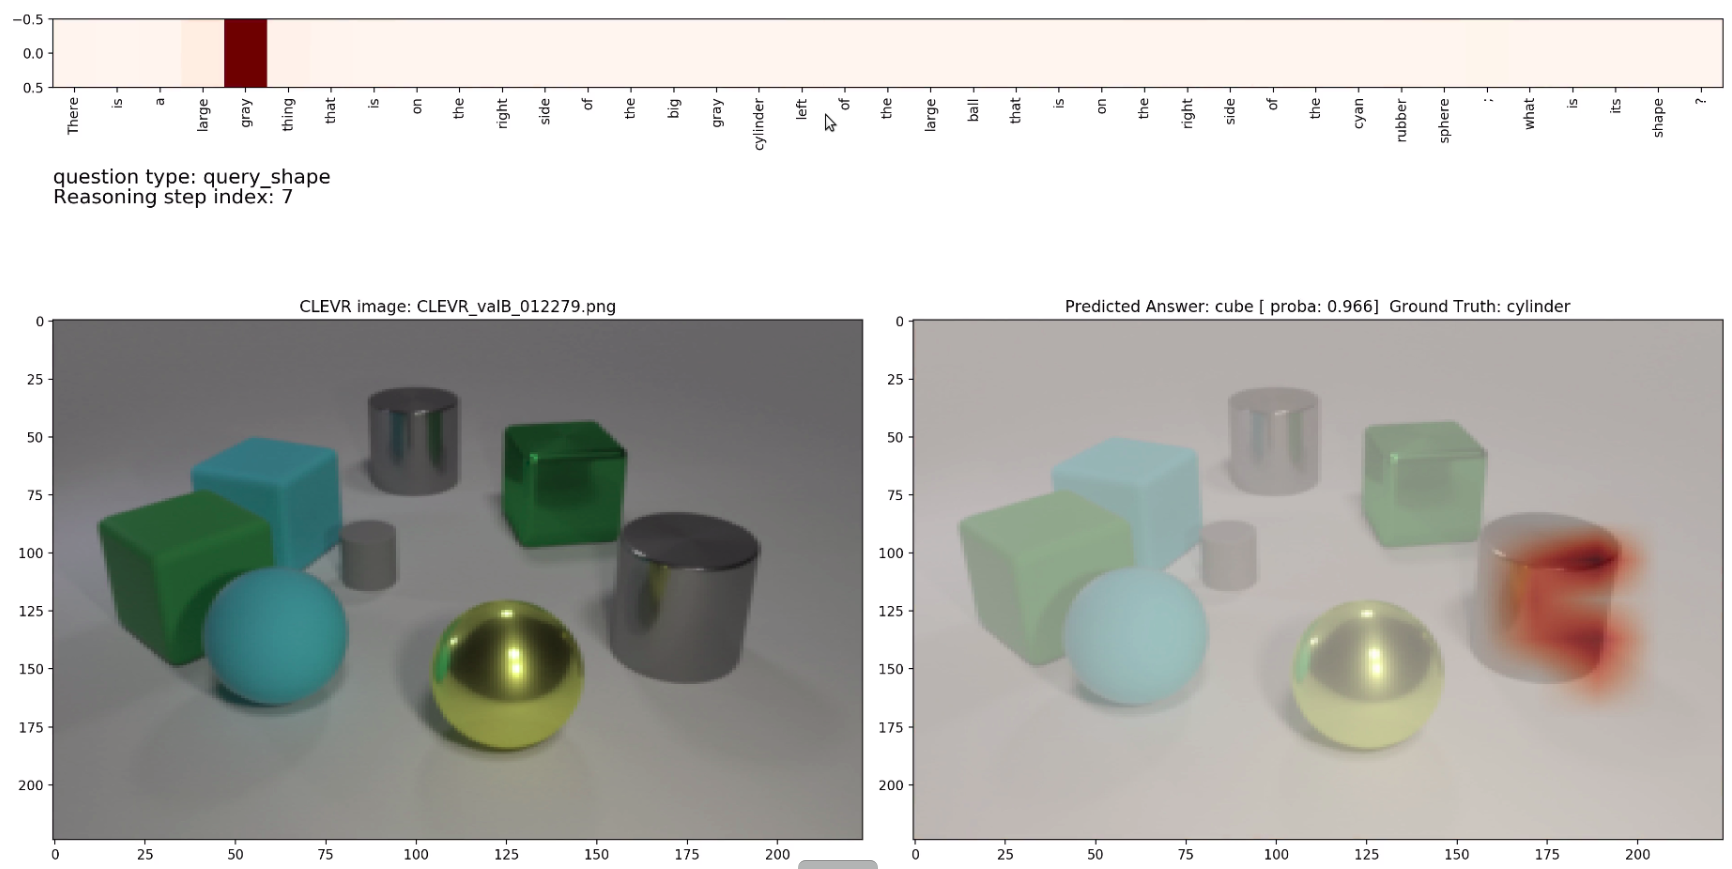
\includegraphics[width=\textwidth]{img/fail_mac_cogent_b_shape.png}
	\caption{The question reads as: \textit{There is a large gray thing that is on the right side of the big gray cylinder left of the large ball that is on the right side if the cyan rubber sphere; what is its shape?}}
	\label{fig:fail_mac_shape}
\end{figure}

\begin{figure}[]
	\centering
	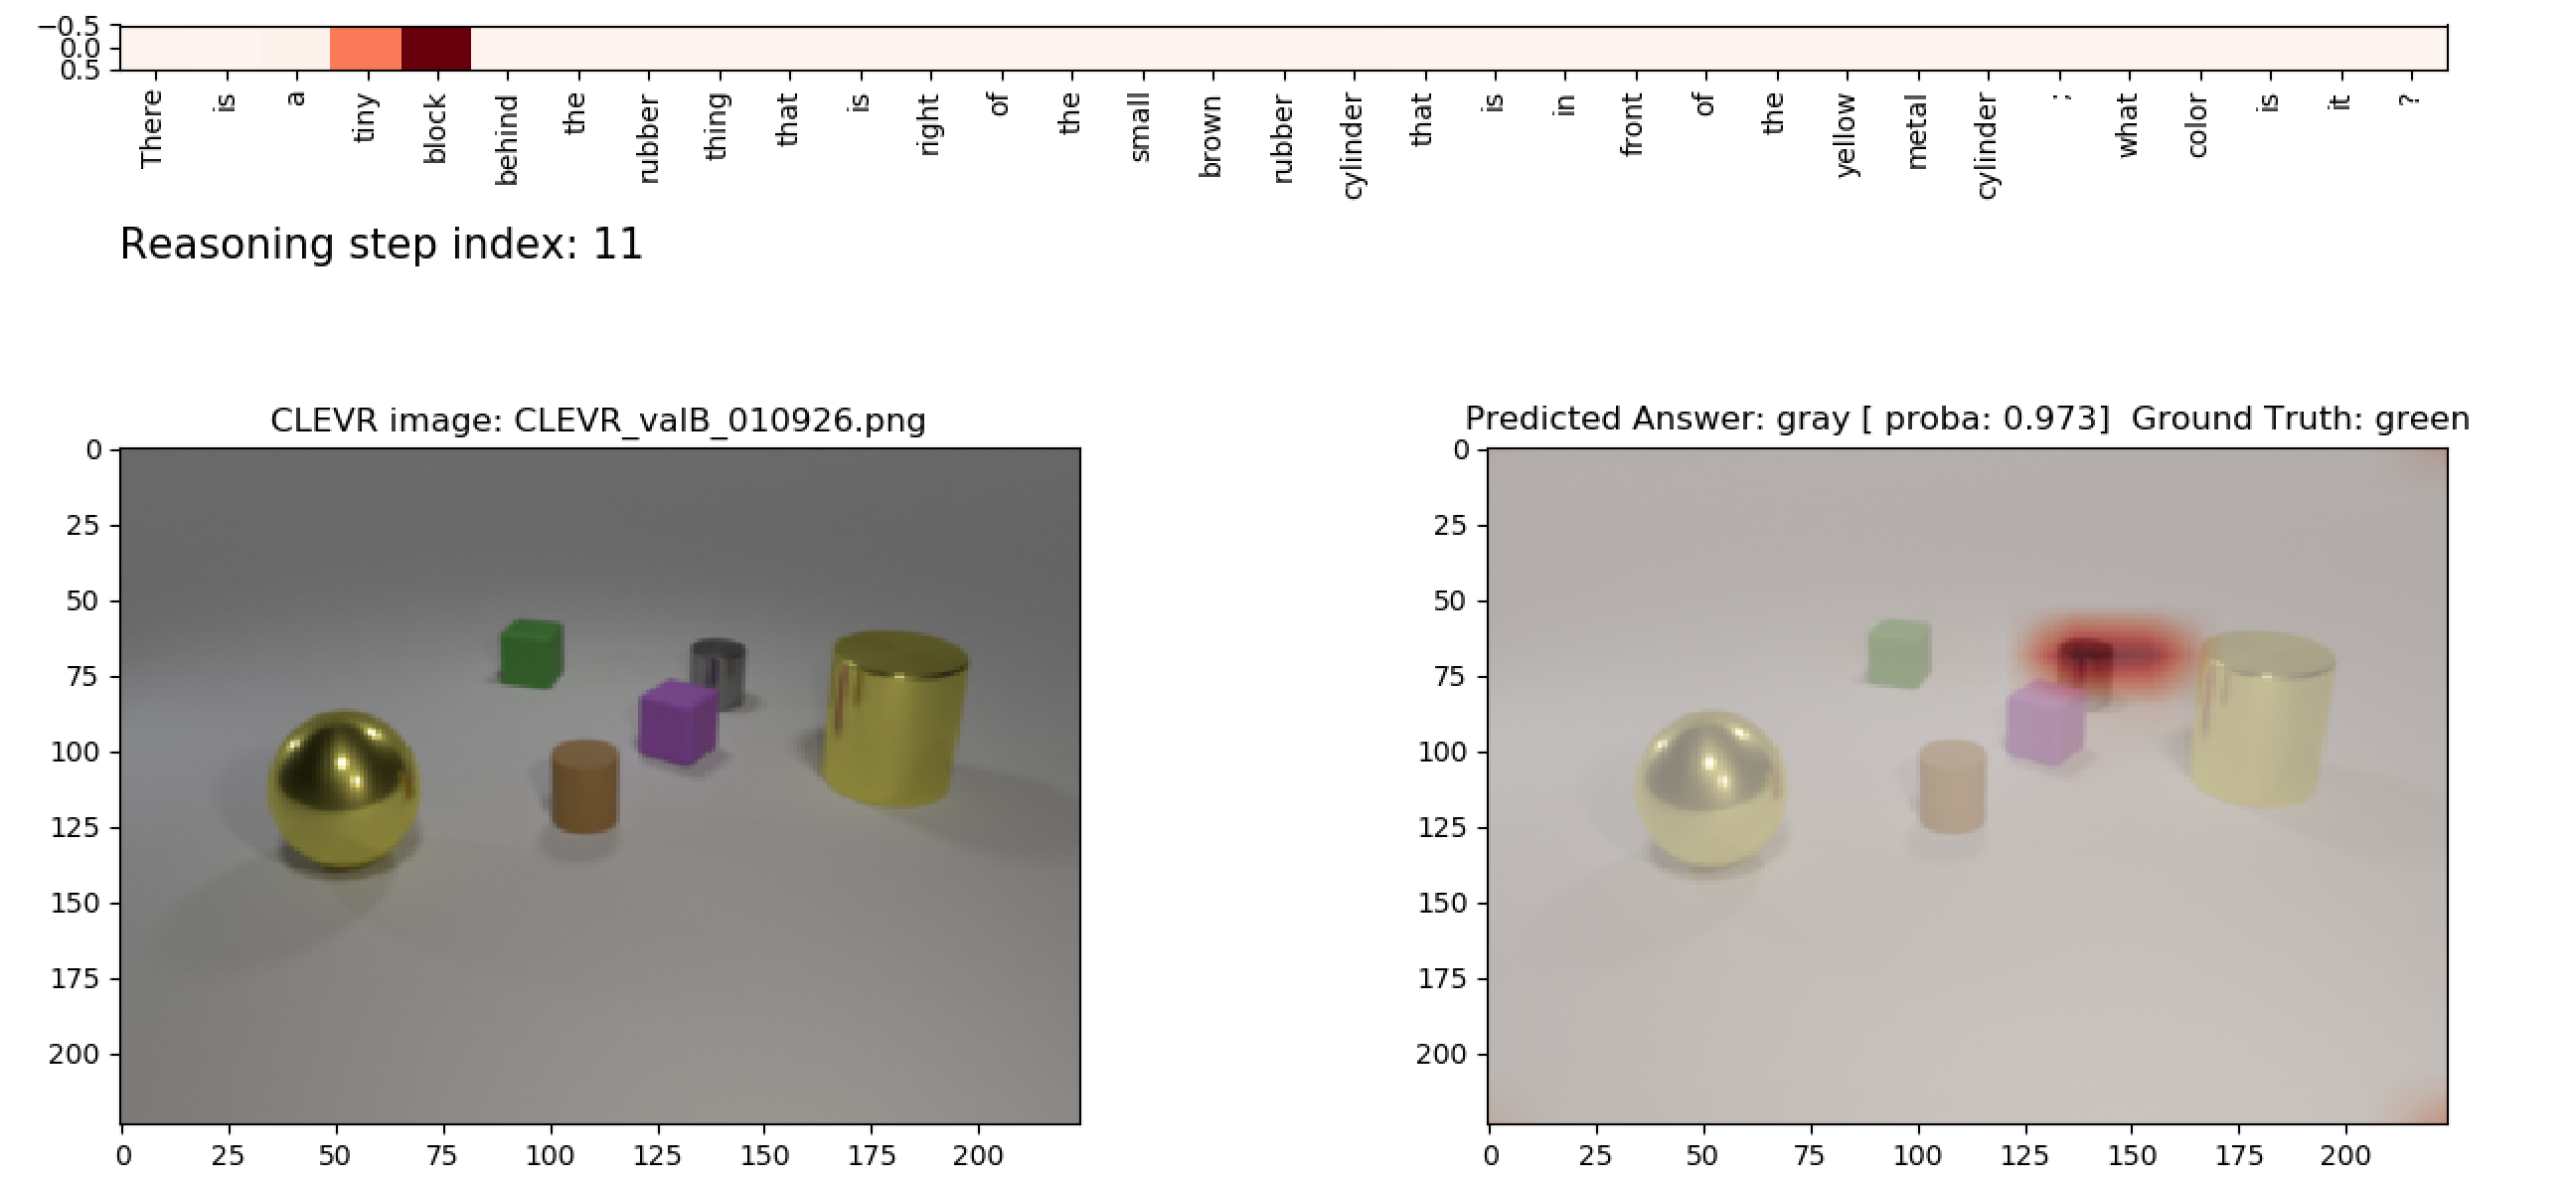
\includegraphics[width=\textwidth]{img/fail_mac_cogent_b_color.png}
	\caption{The question reads as: \textit{There is a tiny block behind the rubber thing that is right if the small brown rubber cylinder that is in front of the yellow metal cylinder; what color is it?}}
	\label{fig:fail_mac_color}
\end{figure}

Those examples indicate that MAC did not correctly separate the concept of shape from the concept of color, but have a better understanding of the colors (as it found the object of interest in \fig{fig:fail_mac_shape} by its color). This could come from that fact that the shape \textit{sphere} is associated with all possible colors in the dataset. 

%
%\newpage
\bibliographystyle{alpha}
\bibliography{vigil_bibliography}


\end{document}
